\begin{surferIntroPage}{Superficies Recordistas}{record_chmutovoktic}{Superf\'icies Recordistas Mundiais}
    Uma superf\'icie diz-se \emph{n\~ao singular} ou \emph{lisa} quando n\~ao tem quaisquer v\'ertices (chamamos a esses pontos  \emph{singularidades}). S\~ao exemplos de superf\'icies lisas a esfera ou o toro, as duas primeiras figuras abaixo.  
   \'E quase certo obtermos uma superf\'icie lisa quando escolhemos uma ao acaso.
 \begin{center}
      \vspace{-0.2cm}
      \begin{tabular}{@{}c@{}c@{}c@{\quad}c@{}c@{}c@{}c@{}}
        \begin{tabular}{@{}c@{}}
          lisa:
        \end{tabular}
        &
        \begin{tabular}{@{}c@{}}
          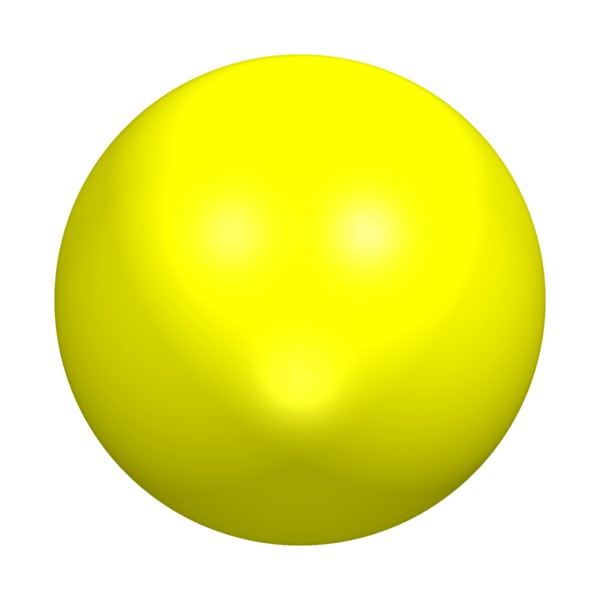
\includegraphics[width=1.1cm]{kugel}
        \end{tabular}
        &
        \begin{tabular}{@{}c@{}}
          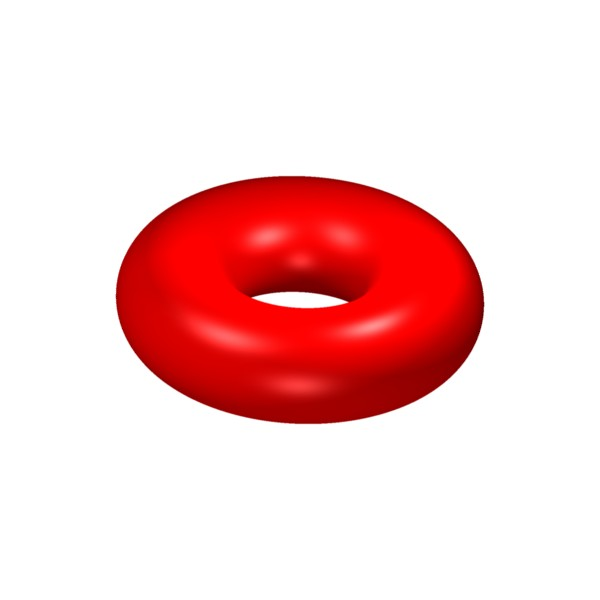
\includegraphics[width=1.1cm]{torus}
        \end{tabular}
        &
        \begin{tabular}{@{}c@{}}
          muitas\\
          singularidades:
        \end{tabular}
        &
        \begin{tabular}{c@{}@{}}
          
\includegraphics[width=1.1cm]{kummer}
        \end{tabular}
        &
        \begin{tabular}{c@{}@{}}
          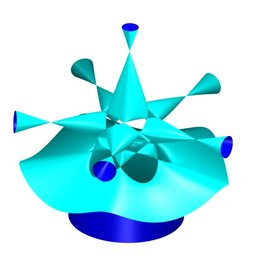
\includegraphics[width=1.1cm]{togliatti}
        \end{tabular}
        &
        \begin{tabular}{c@{}@{}}
          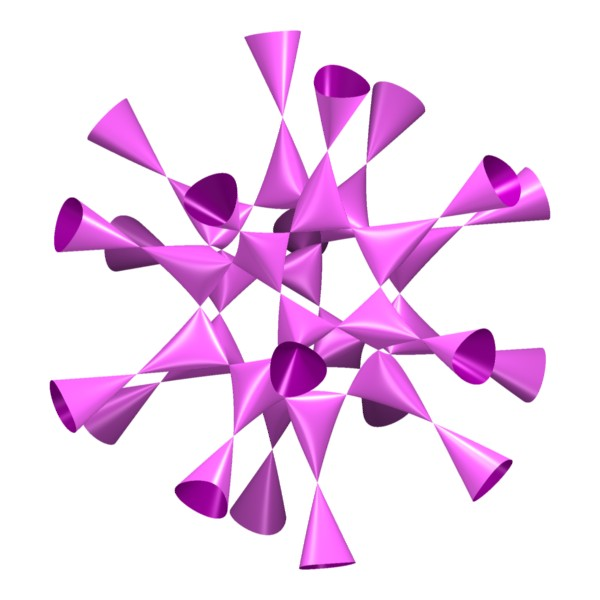
\includegraphics[width=1.1cm]{barth_sextic}
        \end{tabular}
      \end{tabular}
    \end{center}
    \vspace{-0.2cm}
Assim, uma superf\'icie com singularidades \'e mais especial e as singularidades s\~ao os seus pontos mais interessantes. As superf\'icies obtidas com o programa SURFER s\~ao definidas por polin\'omios. A maior pot\^encia de um polin\'omio diz-se o seu grau. Os matem\'aticos tentam descobrir quantas singularidades pode ter uma superf\'icie de um determinado grau $d$.
   Representamos este n\'umero por $\mu(d)$.

 Acontece que este n\'umero $\mu(d)$ \'e muito dif\'icil de calcular.
Para $d=1,2,3,4$, $\mu(d)$ \'e conhecido desde o s\'eculo XIX, mas  para $d=5$  este n\'umero s\'o foi identificado em 1980, e para $d=6$ s\'o em $1996$.   Para $d \ge 7$, $\mu(d)$ \'e ainda desconhecido.
  
    Cada novo recorde mundial para um $\mu(d)$ \'e um  resultado parcial importante. Provavelmente teremos que esperar muito tempo at\'e se  resolver completamente este  problema para qualquer valor arbitr\'ario $d$.\\  Alguns resultados conhecidos:
    
   \begin{center}
      \begin{tabular}{r|cccccccc|c}
        $d$ & $1$ & $2$ & $3$ & $4$ & $5$ & $6$ & $7$ & $8$ & $d$\\
        \hline
        \hline
        \rule{0pt}{1.2em}$\mu(d)\ge$ & $0$ & $1$ & $4$ & $16$ & $31$ & $65$ &
        $99$ & $168$ & 
        $\approx \frac{5}{12}d^3$\\[0.3em]
        \hline
        \rule{0pt}{1.2em}$\mu(d)\le$ & $0$ & $1$ & $4$ & $16$ & $31$ & $65$ &
        $104$ & $174$ & $\approx \frac{4}{9}d^3$
      \end{tabular}
    \end{center}
\end{surferIntroPage}
